\subsection{Estratégias de Segmentação}

A indexação vetorial exige a discretização de documentos longos em unidades menores, denominadas \textit{chunks}. A definição da granularidade dessa discretização envolve um compromisso crítico entre a densidade de informação relevante (sinal) e a inclusão de informações periféricas irrelevantes (ruído).

Conforme \citet{zhang2024_chunking}, essa segmentação impacta diretamente a probabilidade de recuperação $P(Z|q)$ de um trecho $Z$ dada uma consulta $q$, manifestando-se de duas formas antagônicas:

\begin{itemize}
  \item \textbf{Granularidade Fina (\textit{Small Chunks}):} Maximiza a proporção de sinal e a similaridade de cosseno ao isolar fatos específicos. Contudo, corre o risco de fragmentar o contexto, rompendo correferências e unidades de raciocínio essenciais para a interpretação correta da informação.
  \item \textbf{Granularidade Grossa (\textit{Large Chunks}):} Preserva o contexto global e as dependências semânticas. No entanto, o vetor resultante torna-se uma média semântica de um texto extenso, diluindo a especificidade da informação buscada. Além de prejudicar a recuperação vetorial, o excesso de ruído contextual degrada a capacidade de atenção do modelo de linguagem durante a síntese da resposta \citep{liu2023lostmiddlelanguagemodels}.
\end{itemize}

Para equilibrar essa balança e otimizar a recuperação, a literatura propõe duas abordagens principais de segmentação. A primeira foca em regras mecânicas, enquanto a segunda utiliza a própria distribuição semântica dos dados.
\subsubsection{Segmentação Recursiva e Janelas Deslizantes}

A abordagem padrão discretiza o texto baseando-se em delimitadores sintáticos (parágrafos, quebras de linha) e um limite fixo de caracteres $L$.

A principal limitação teórica deste método é a imposição de fronteiras arbitrárias que podem seccionar sentenças ou argumentos lógicos nas bordas (\textit{boundary loss}). Para mitigar a perda de informação nessas extremidades, aplica-se a técnica de Janela Deslizante com Sobreposição (\textit{Overlap}). Seja $C_i$ o $i$-ésimo \textit{chunk} de comprimento $L$ e $O$ o tamanho da sobreposição, o início do \textit{chunk} $C_{i+1}$ é deslocado por $L - O$ em relação a $C_i$.

\begin{figure}[ht]
  \centering
  \includesvg[width=0.5\columnwidth]{figuras/overlap}
  \caption{Processo de segmentação com janela deslizante.}
  \label{fig:chunking_overlap}
\end{figure}

A Figura \ref{fig:chunking_overlap} ilustra essa redundância intencional. O parâmetro $O > 0$ garante a continuidade semântica e assegura que termos localizados no final de um segmento possuam contexto à direita na janela subsequente. Neste trabalho, definiram-se empiricamente janelas com $O$ proporcional a 20\% de $L$.

Contudo, mesmo com a sobreposição, a segmentação recursiva permanece ``cega'' ao significado do texto. Para contornar essa falha estrutural, modelos mais avançados adotam estratégias estatísticas de corte.

\subsubsection{Segmentação Semântica}

Em contraste com a métrica fixa de caracteres, a Segmentação Semântica propõe que as quebras ocorram apenas quando há uma mudança significativa de tópico. O método baseia-se na premissa geométrica de que mudanças de assunto correspondem a grandes distâncias angulares no espaço vetorial.

O algoritmo opera calculando a similaridade semântica $sim(s_t, s_{t+1})$ entre sentenças sequenciais. Formalmente, define-se uma fronteira de \textit{chunk} no índice $t$ se a dissimilaridade exceder um limiar crítico $\tau$:

\begin{equation}
  1 - sim(s_t, s_{t+1}) > \tau,
\end{equation}

onde $\tau$ é tipicamente definido como um percentil da distribuição de distâncias do documento.

Conforme ilustrado na Figura \ref{fig:semantic_chunking}, esta abordagem agrupa sentenças semanticamente coesas (como $S_1$, $S_2$ e $S_3$), minimizando a variância intra-\textit{chunk}. A transição entre $S_3$ e $S_4$ apresenta uma similaridade ($0.21$) consideravelmente inferior ao limiar definido (neste exemplo, $\tau = 0.5$). Essa queda brusca provoca a quebra geométrica do documento e marca o início de um novo \textit{chunk}. Ao detectar essa fronteira natural do tópico e realizar o corte estrutural, o sistema teoricamente maximiza a relevância do contexto recuperado, evitando a inserção de assuntos desconexos no \textit{prompt} do modelo gerador.

\begin{figure}[!htb]
  \centering
  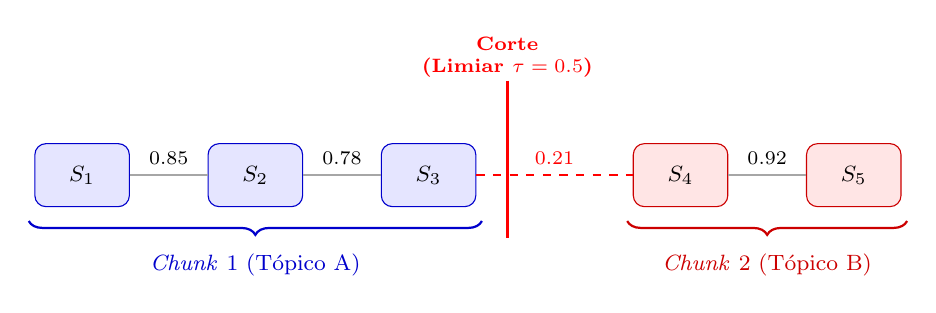
\begin{tikzpicture}[>=stealth, auto, node distance=2.2cm]

    % Estilo dos nós (sentenças)
    \tikzstyle{sentenca}=[draw, rounded corners, minimum width=1.2cm, minimum height=0.8cm, font=\footnotesize]

    % Sentenças do Chunk 1
    \node[sentenca, fill=blue!10, draw=blue!80!black] (s1) {$S_1$};
    \node[sentenca, fill=blue!10, draw=blue!80!black, right of=s1] (s2) {$S_2$};
    \node[sentenca, fill=blue!10, draw=blue!80!black, right of=s2] (s3) {$S_3$};

    % Sentenças do Chunk 2 (maior distância para ilustrar a quebra)
    \node[sentenca, fill=red!10, draw=red!80!black, right of=s3, node distance=3.2cm] (s4) {$S_4$};
    \node[sentenca, fill=red!10, draw=red!80!black, right of=s4] (s5) {$S_5$};

    % Conexões de Alta Similaridade
    \draw[thick, gray!70] (s1) -- node[above, font=\scriptsize, text=black] {0.85} (s2);
    \draw[thick, gray!70] (s2) -- node[above, font=\scriptsize, text=black] {0.78} (s3);
    \draw[thick, gray!70] (s4) -- node[above, font=\scriptsize, text=black] {0.92} (s5);

    % Conexão de Baixa Similaridade (Onde ocorre a quebra)
    \draw[thick, red, dashed] (s3) -- node[above, font=\scriptsize, text=red] {0.21} (s4);

    % Linha indicadora de Corte
    \draw[very thick, red] (5.4, 1.2) -- (5.4, -0.8);
    \node[red, font=\bfseries\scriptsize, align=center] at (5.4, 1.5) {Corte\\(Limiar $\tau = 0.5$)};

    % Chaves mostrando os Chunks finais
    \draw[decorate, decoration={brace, amplitude=5pt, mirror}, thick, blue!80!black]
    ([xshift=-2pt, yshift=-5pt]s1.south west) -- ([xshift=2pt, yshift=-5pt]s3.south east)
    node[midway, below=8pt, font=\footnotesize] {\textit{Chunk} 1 (Tópico A)};

    \draw[decorate, decoration={brace, amplitude=5pt, mirror}, thick, red!80!black]
    ([xshift=-2pt, yshift=-5pt]s4.south west) -- ([xshift=2pt, yshift=-5pt]s5.south east)
    node[midway, below=8pt, font=\footnotesize] {\textit{Chunk} 2 (Tópico B)};

  \end{tikzpicture}
  \caption{Abstração do processo de Segmentação Semântica.}
  \label{fig:semantic_chunking}
\end{figure}
